\documentclass{beamer}
\usepackage{verbatim}

\begin{document}

\begin{comment}
%1) 5-state example
%	-more about limit cycles, steady states, components
%	-biological correspondance
%	-in-depth 3-limit cycle
\begin{frame}
 \frametitle{Example with 5 States}
\begin{figure}
    \centering
    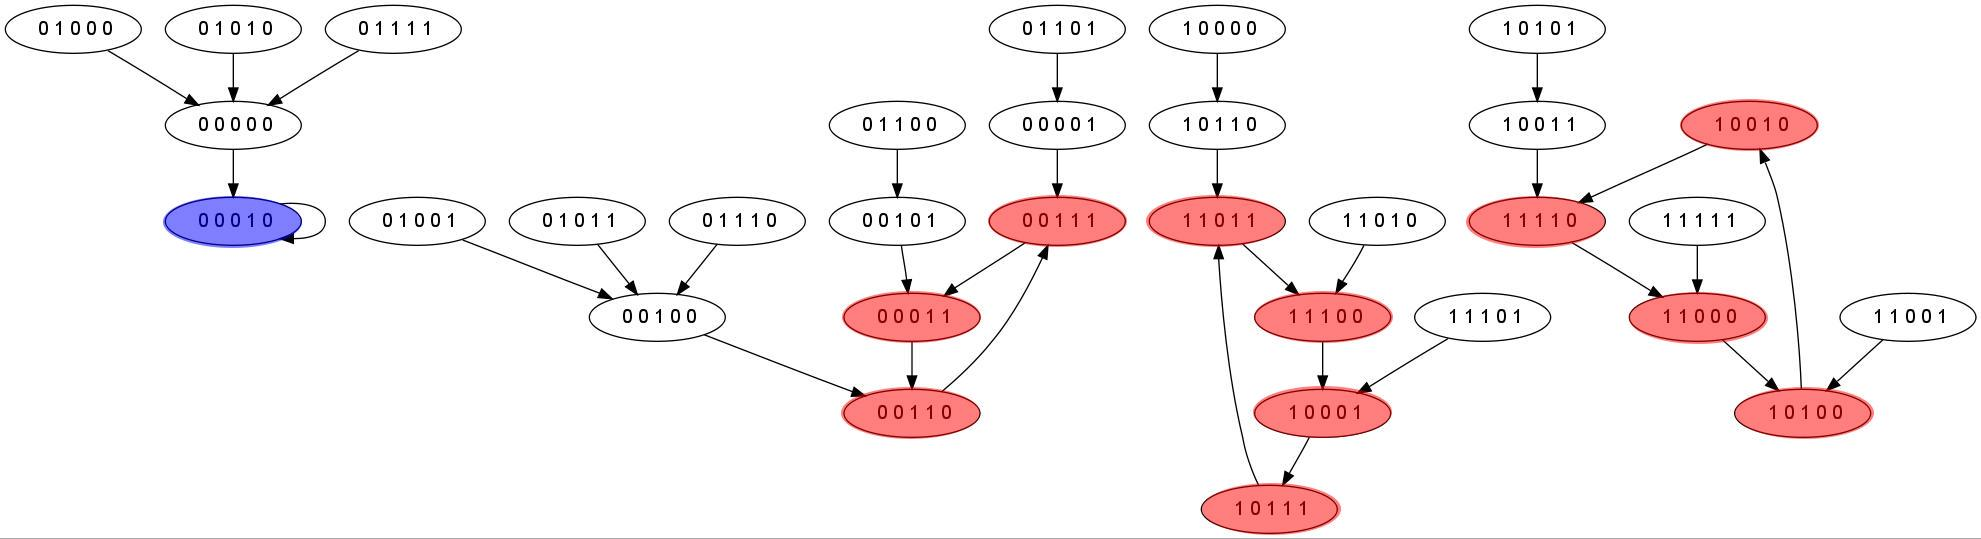
\includegraphics[width = 4in]{5states-1.jpg}
\end{figure}
\begin{itemize}
    \item Can see: 1 fixed point, 1 3-limit cycle, 2 4-limit cycles - total of 4 components \\
    \item Fixed point: point that is mapped to itself by a function \\
    \item Limit cycle: set of points such that all other points in the component approach the cycle \\
\end{itemize}
%Equations that generated this were: $f1 = x1;$ $f2 = x1*x4;$ $f3 = x1 + x5*(1 + x1) + x3;$ $f4 = 1 + x2;$ $f5 = x2*x3 + x3*x4 + (1+x4)*(1+x2)*x5$.
\end{frame}

\begin{frame}
 \frametitle{Closer Look at 3-Limit Cycle}
\begin{figure}
    \centering
    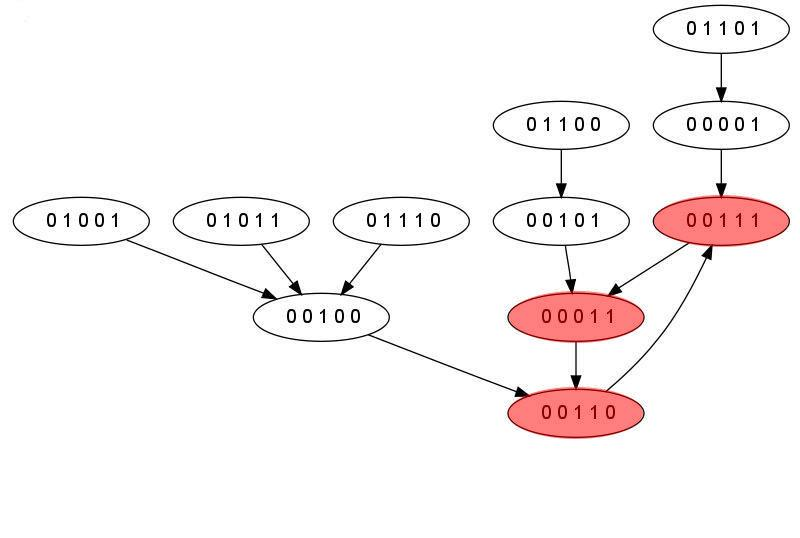
\includegraphics[width = 0.5\textwidth]{limitcycle-1.jpg}
\end{figure}
\begin{itemize}
\item Usually want large components with short cycles
\item Biological meaning: small perturbations in the system won't make it go off somewhere else
\end{itemize}
\end{frame}\end{comment}

\begin{comment}
%2) Limitations of DVD
%	-1000 states
%	-graph of 9 nodes
\begin{frame}
 \frametitle{What Happens As n Gets Bigger?}
\begin{itemize}
 \item DVD can take a max of 1000 nodes.
 \item Let n = 9. Have to graph $2^9 = 512$ nodes.
\end{itemize}
\begin{figure}
    \caption{9 functions plugged into DVD. There are 9 nodes and 2 states.}
    \centering
    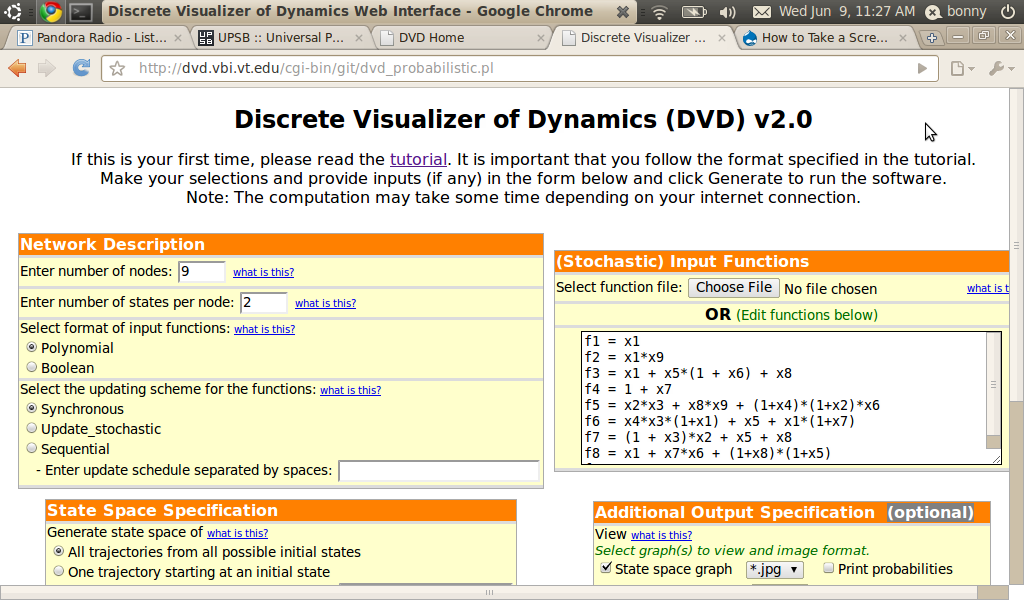
\includegraphics[width = 4in]{dvd1.png}
\end{figure}
\end{frame}

\begin{frame}
\begin{figure}
    \caption{DVD's analysis says that there are 9 components, 4 fixed points of sizes from 2 nodes to 32 nodes.}
    \centering
    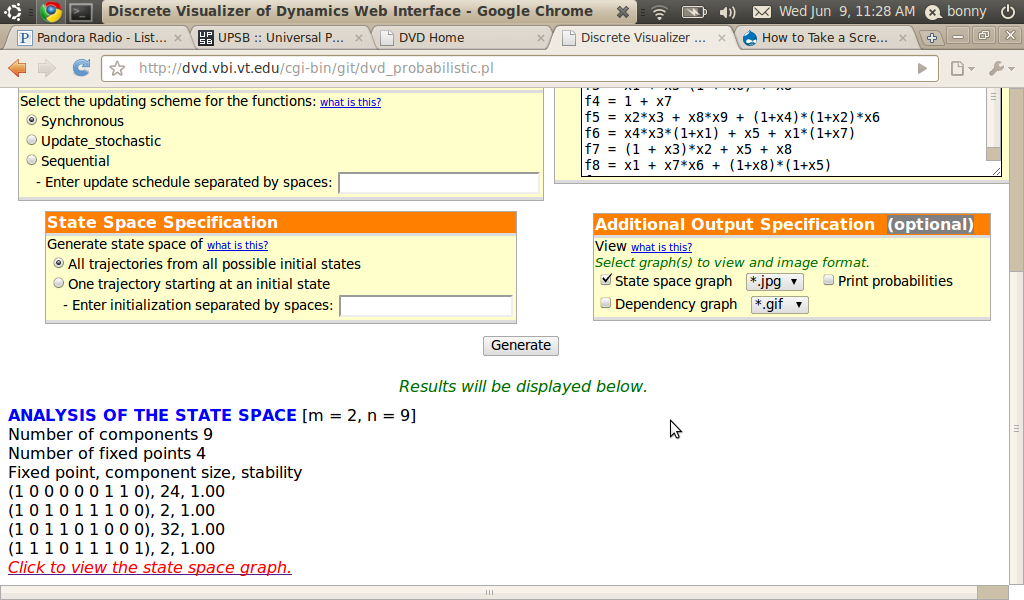
\includegraphics[width = 4in]{dvd2.png}
\end{figure}
\end{frame}
\end{comment}

\begin{frame}
 \frametitle{A Real-Life Wiring Diagram}
\begin{figure}
    \vspace{-10pt}
    \caption{Mammalian cell cycle with at least 60 nodes.}
    \centering
    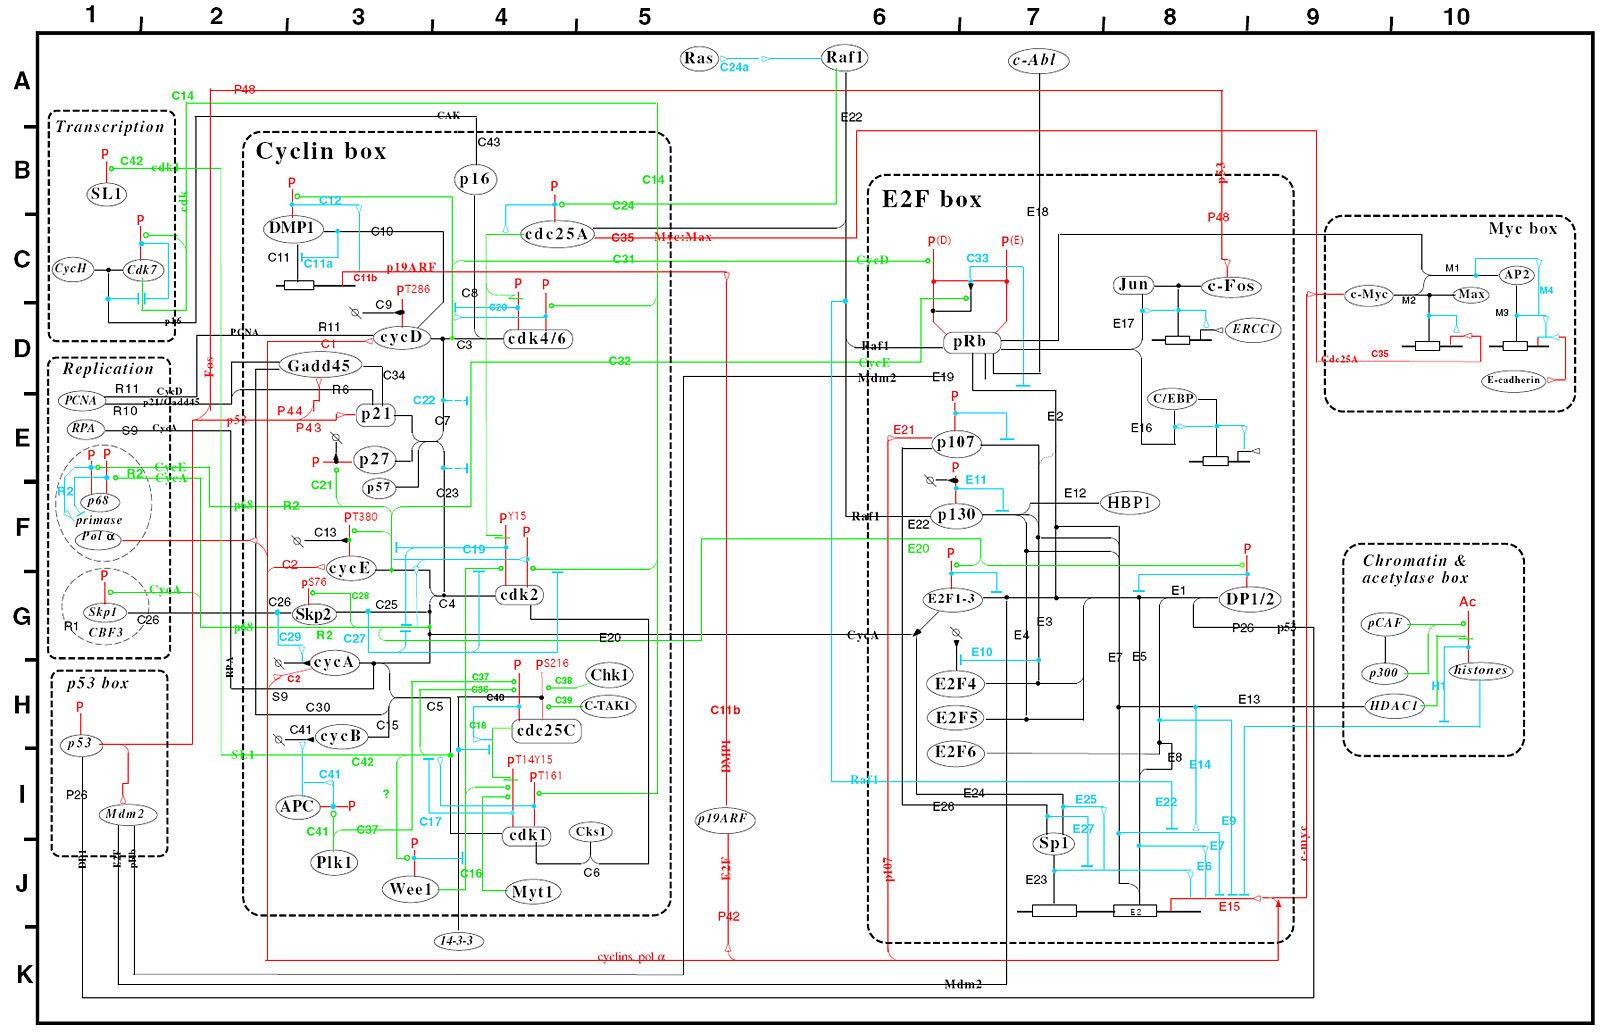
\includegraphics[width = 0.95\textwidth]{hugewiringdiagram.jpg}
    \vspace{-10pt}
\end{figure}
\end{frame}

\begin{frame}
 \frametitle{State Space Diagrams}
\begin{itemize}
 \item $2^{60} \approx 1.2 \times 10^{18}$ states. Let's scale down to $n = 9$ nodes. (DVD online can only take $1000$ states)
 \item Even for $n = 9$, when we try to see the state space graph...
\end{itemize}
\begin{figure}
    \caption{Boolean state space graph, 9 nodes.}
    \centering
    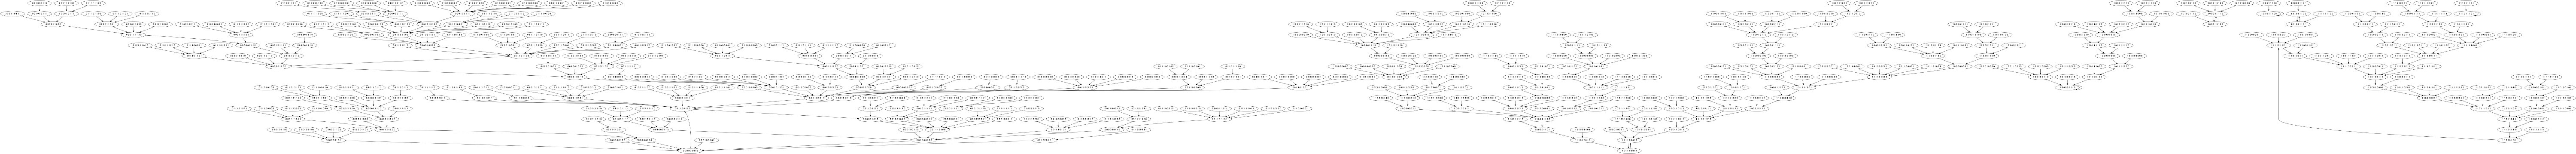
\includegraphics[width = 4in]{9states-1.jpg}
\end{figure}
Impossible to even see the 9 states on one screen!
\begin{figure}
  \centering
  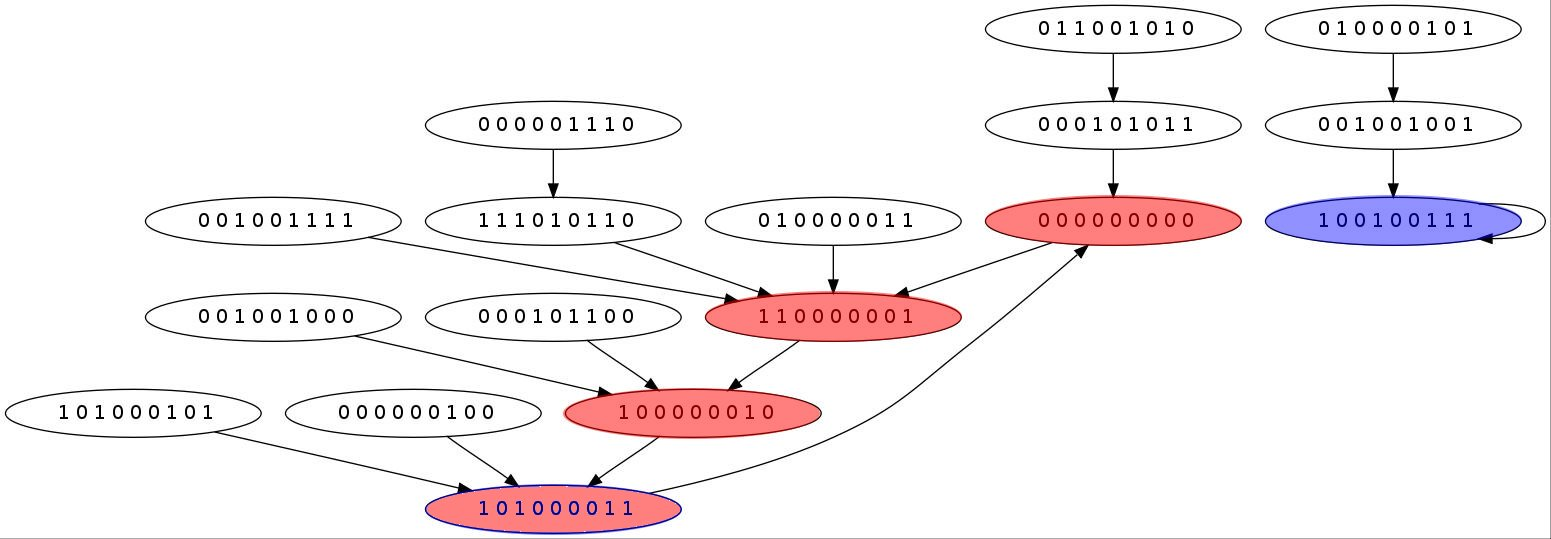
\includegraphics[width=0.8\textwidth]{RandomNetwork.jpg}
  \caption{Cropping of 3\% of graph.}
\end{figure}
\end{frame}

\end{document}
